\chapter{Proteins}
\section[What are proteins?]{What are proteins and why do we care?}
\lettrine[lines=3, lhang=0.25,  nindent=0em, findent=2pt]{\color{Maroon}P}{roteins are\ }
the fundamental machines in biology, performing tasks such as catalysis, transporting molecules, and providing the structural backbone of the cell.
They have crucial roles in the biochemical pathways, so understanding them can lead us to create new and refined drugs or bio-engineered organisms.

%In this chapter I will present the basic vocabulary of protein structures, and give an overview of their biochemistry.

But, how are they created?
The information \marginpar{Protein biosynthesis}
used by the cell to build proteins is encoded in the \DNA.
When the biosynthesis begins, the double helix unfolds, and the genetic contact is translated into \RNA{}.
This new molecule is then transported to the ribosome, the machinery that translates the \RNA{} into functional proteins.

The \DNA is in itself a polymer of four blocks: the bases A, T, G, and C.
\marginpar{Translation}

\todo[inline]{Expand on translation, codons}

\section{The many levels of protein structures}
Proteins are polymers, long chains of amino acids, structured at several levels, depending on which scale we look at them.
In this section, I will present the main descriptions of proteins at different scopes.

\subsection{The amino acids}
Amino acids are the building blocks of proteins.
They are composed of a carboxyl (-$COOH$) and an amine (-$NH_2$) groups, forming the backbone, and a side-chain.
Two examples are illustrated in Figure~\ref{fig:amino_acids}.
\marginpar{Only a few of all amino acids appear in the \DNA.}
\DNA{} usually codifies up to twenty different species, but at least 500 are known to occur naturally \citep{500_amino_acids}.
The differences between most of them are only on the side chain\footnote{The amino acid proline's side-chain has a ring connecting with the amine in the backbone.}.

The side chains are the group responsible for the specific physico-chemical properties of the compound, such as hydrophobicity, pH, or electrostatic charge.

The backbone can polymerise, bonding with other amino acids and forming a long chain.
Having a common backbone means that in principle, any amino acid can be connected to any other, which gives proteins a lot of flexibility:
for a protein of length $L$ there are $20^L$ possible combinations. %$20/19 (20^L - 1)$

\begin{figure}
\centering
\hfil %
\subcaptionbox{Glutamine (Q) \label{subfig:aminoQ}}{\begin{tikzpicture}
    \node[anchor=south west,inner sep=0] (image) at (0,0) {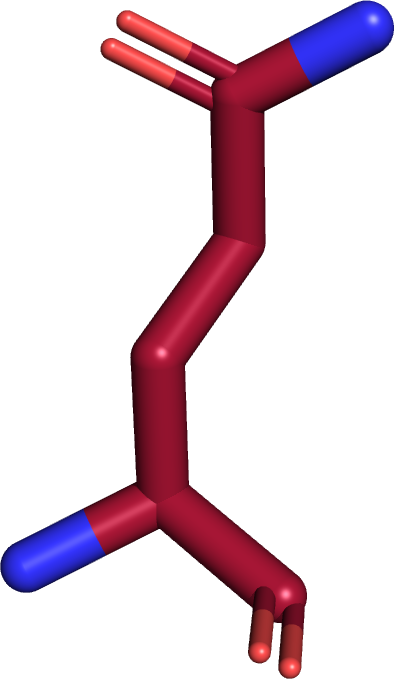
\includegraphics[width=0.25\columnwidth]{bioinfo/figures/amino_acid_Q}};
    \begin{scope}[x={(image.south east)},y={(image.north west)}]
    	\draw[Maroon, thick] (-0.05, -0.05) rectangle (0.85,0.3);
    	\draw[RoyalBlue, thick, dashed] (0.2, 0.35) rectangle (1.05, 1.05);
        %\draw[help lines,xstep=.1,ystep=.1] (0,0) grid (1,1);
        %\foreach \x in {0,1,...,9} { \node [anchor=north] at (\x/10,0) {0.\x}; }
        %\foreach \y in {0,1,...,9} { \node [anchor=east] at (0,\y/10) {0.\y}; }
    \end{scope}
\end{tikzpicture}
} %
\hfil %
\subcaptionbox{Tyrosine (Y) \label{subfig:aminoY}}{\begin{tikzpicture}
    \node[anchor=south west,inner sep=0] (image) at (0,0) {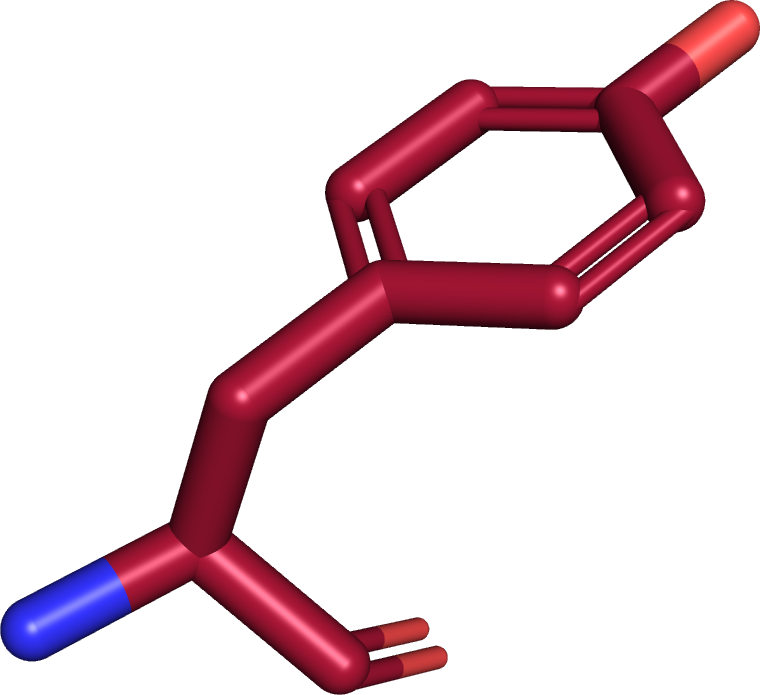
\includegraphics[width=0.45\columnwidth]{bioinfo/figures/amino_acid_Y}};
    \begin{scope}[x={(image.south east)},y={(image.north west)}]
	    \draw[Maroon, thick] (-0.05, -0.05) rectangle (0.6,0.3);
 	    \draw[RoyalBlue, thick, dashed] (0.2, 0.35) rectangle (1.05, 1.05);
        %\draw[help lines,xstep=.1,ystep=.1] (0,0) grid (1,1);
        %\foreach \x in {0,1,...,9} { \node [anchor=north] at (\x/10,0) {0.\x}; }
        %\foreach \y in {0,1,...,9} { \node [anchor=east] at (0,\y/10) {0.\y}; }
    \end{scope}
\end{tikzpicture}
} %
\hfil %
\caption{Two amino acids as appear in proteins.
The \textcolor{Maroon}{maroon}, solid rectangle indicates the backbone, common to all amino acids; and the \textcolor{RoyalBlue}{blue} dashed the side chain, that determines the specific chemical properties.}\label{fig:amino_acids}
\end{figure}

\subsection{Primary structure or sequence}
The amino acids can connect to each other through the peptide bond, forming a chain.
The \emph{primary structure} is the sequence of amino acids as encoded in the \DNA:
\begin{center}
\texttt{ALA ARG ILE ASN GLY ARG GLU ILE ASN VAL THR LYS LYS}
\end{center}

%\missingfigure{peptide bond}

This is the easiest to obtain experimentally since the advent of next-generation sequencing techniques.
These experiments read the \DNA{} of the organism, that can be translated into proteins.
The collection of all protein sequences of an organism is the \emph{proteome}.


\subsection{Secondary structure}
The polypeptide chains are locally organised in motifs stabilised by hydrogen bonds.
The most common is the $\alpha$-helix, \marginpar{$\alpha$} shown in Figure~\ref{subfig:alpha}, where the hydrogen bonds are formed between the backbone oxygen of one residue, and the hydrogen of the amine group, four residues beyond, and continued in a regular pattern, forcing the backbone to twist into a helix.
The same bond is possible with residues that are closer -- two or three -- or further  -- five residues, the $\pi$ helix -- but are less common.

The second most common arrangement is the $\beta$-sheet  \marginpar{$\beta$} depicted in Figure~\ref{subfig:beta}, where approximately extended chains are placed next to each other and bonds are formed between juxtaposed residues.


\begin{figure}[tbp]
	\centering
	\subcaptionbox{$\alpha$-helix\label{subfig:alpha}}{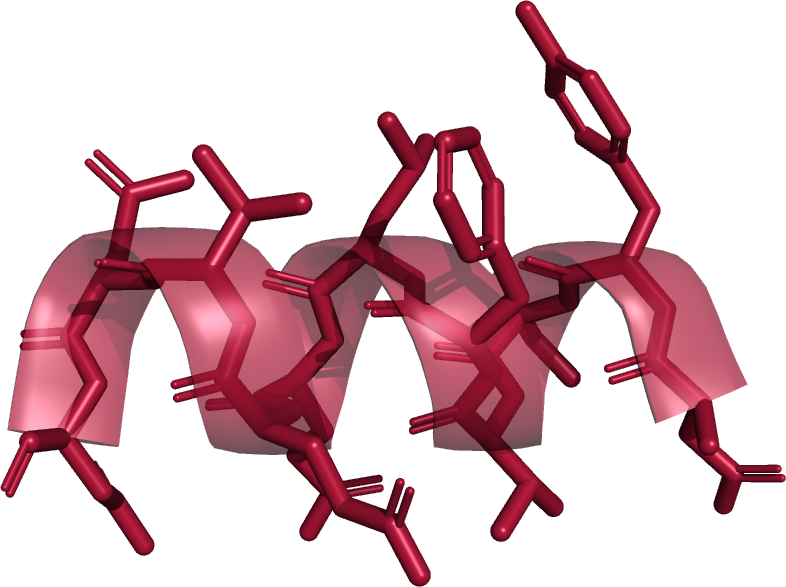
\includegraphics[width=0.9\textwidth]{bioinfo/figures/helix}}\\
	\subcaptionbox{$\beta$-sheet\label{subfig:beta}}{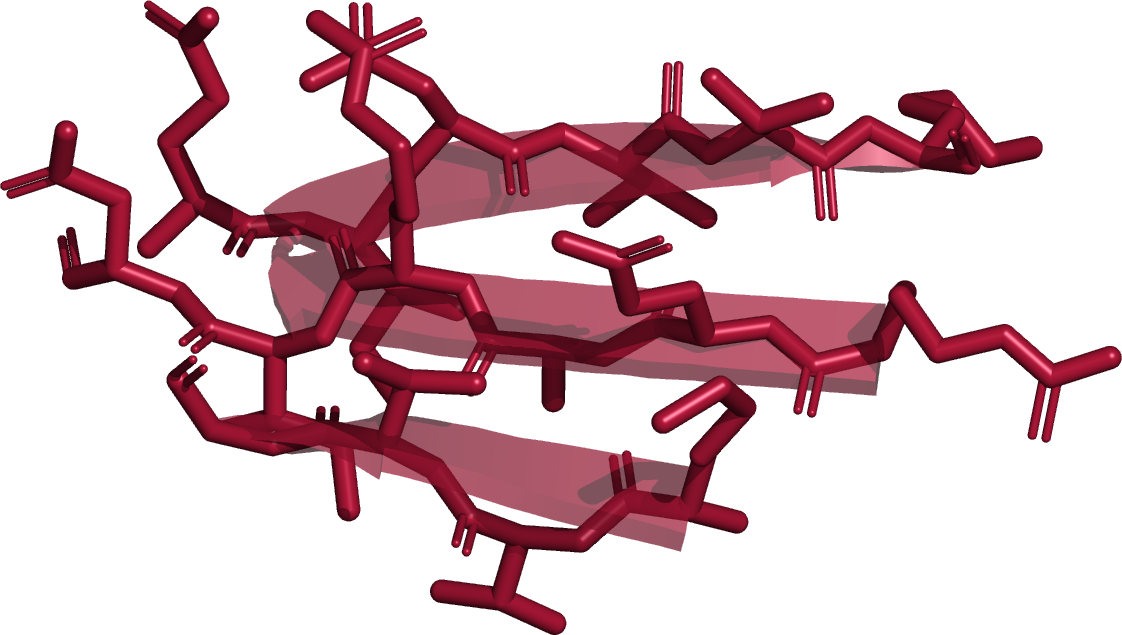
\includegraphics[width=0.9\textwidth]{bioinfo/figures/beta}}
	\caption{The two most frequent secondary structure elements.}\label{fig:alpha_beta}
\end{figure}


\subsection{Tertiary structure}
Once the chain is locally stabilised by the hydrogen bonds it folds into a compact structure.
The spatial arrangement of the secondary structure elements is the \emph{tertiary structure.}
One example is the chain A of the protein \texttt{4V0B}, in Figure~\ref{fig:tertiary}.

\begin{figure}[htb]
\centering
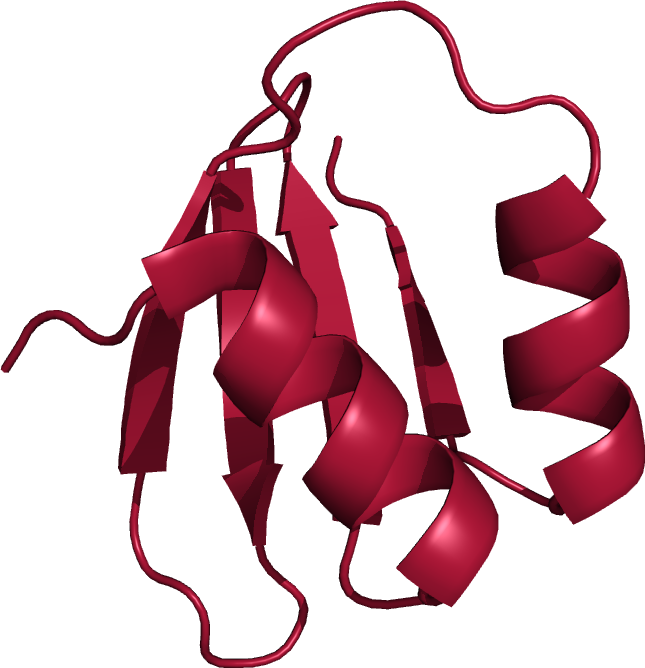
\includegraphics[width=0.8\textwidth]{bioinfo/figures/tertiary}
\caption{The tertiary structure of chain B of the protein \texttt{4V0B}.}\label{fig:tertiary}
\end{figure}

\subsection{Quaternary structure}
Proteins do not always work alone, but they form complexes composed of several chains.
The relative arrangement of each chain is the quaternary structure.

\begin{figure}[htb]
\centering
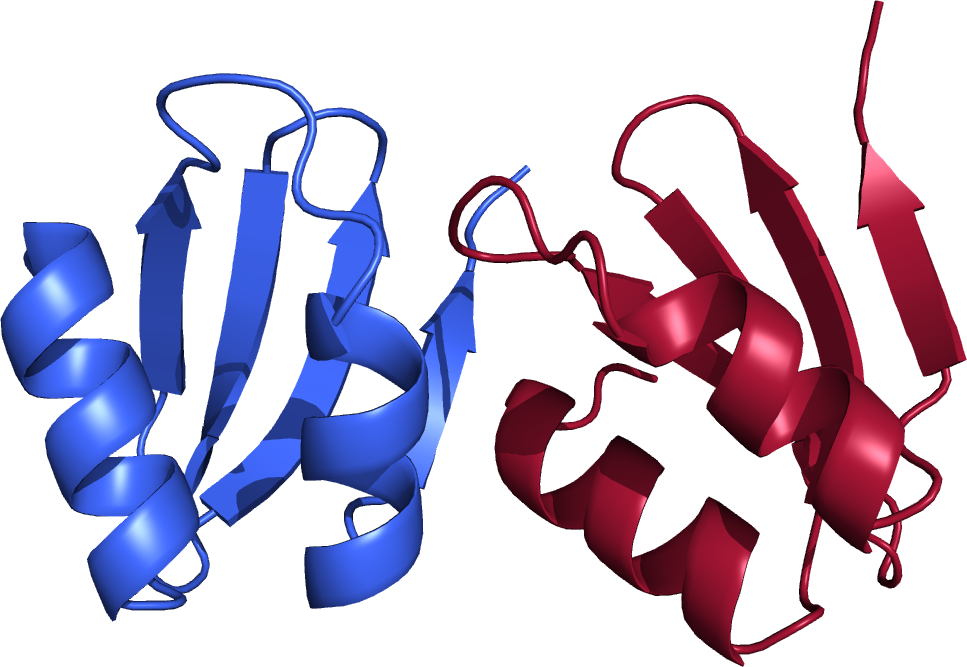
\includegraphics[width=0.8\textwidth]{bioinfo/figures/quaternary}
\caption{Quaternary structure of the chains A and B of the protein \texttt{4V0B}.}\label{fig:quaternary}
\end{figure}

%\subsection{Quintenary structure} %?
\section{Protein biochemistry}

Experiments by \citet{fold_graciously} show that proteins placed in the right medium of pH and temperature will unfold into a random coil, with no trace of tertiary nor secondary structure.
When restored to physiological conditions, they will refold into its natural shape, recovering its original biological and chemical properties.
As long as the protein is chemically unaltered, it will recover the tertiary structure independently of the folding machinery of the cell.
\marginpar{Dogmas that govern protein folding}
This was codified as Anfinsen's dogma: under physiological conditions, the primary structure of globular proteins determines the secondary and tertiary structures, and thus, its function, independently of the cell's machinery \citep{Anfinsen_dogma}.
Typically, the fully folded state is reached in the order of milliseconds to seconds.
The hypothesis has a few exceptions, namely: fibrous proteins, prions -- which are proteins that have an alternative but non-functional stable tertiary structure\footnote{Infamous cause of the mad cows disease.} --  aggregating proteins -- where the individual proteins bind to each other forming large and non-functional structures\footnote{For example, the cause of Alzheimer and Multiple Sclerosis} -- and large, multi-domain proteins.
A reasonable hypothesis is that a priori, the native conformation seems to be the state in the lowest energy, and the random coil is just rolling down the energy landscape.

Cyrus Levinthal \marginpar{Levinthal's paradox} noted that, for every amino acid, a protein has two main degrees of freedom corresponding to the torsion of the backbone, plus one more for the rotation of the side chain.
This gives us a configuration space of the order of $10^{2L}$ for a protein of $L$ residues, but the kinematics suggest that it only has time to sample $10^8$ conformations, an exponentially tiny fraction for proteins of typical length.

Levinthal suggested two corrections:
\begin{itemize}
	\item The native conformation is not necessarily the one of minimum energy, but a local meta-stable minimum with a deep enough well that it is stable.
	For most proteins, this is not very deep, around 10-\SI{15}{\kilo cal/\mol}.
	\item The native conformation must be kinematically accessible, possibly guided by local interactions that partially fold the protein.
	In other words, the energy landscape of protein folding presents a wide funnel from the unfolded state to its near-native conformation, which allows for a rapid transition.
\end{itemize}

%These corrections are supported by experiments showing that a certain enzyme only folds at temperatures around 37 C, but it is completely stable up to 90 C.
%Furthermore, the same enzyme produced by an organism that lives at colder temperatures is shown to require lower temperatures for renaturation, but it is still stable up to 90 C.
%The order of events greatly influences the kinetics of folding.

%\FloatBarrier
%\subsection{The protein backbone}
\subsection{The hydrophobic effect}
Water molecules are electric dipoles with a partial negative charge on the oxygen, and a partial positive charge on the hydrogens.
This introduces an electrostatic interaction between molecules in bulk of water, that self-organises to form a network of hydrogen bonds.
Any non-polar molecule submerged in water will disrupt this network of bonds.
To preserve as many energy-favourable hydrogen bonds the water molecules near the boundary can reorient themselves, forming a pocket around the hydrophobic substance in the process.
The degrees of freedom for the boundary is restricted, so the entropy -- and consequently the free energy -- is reduced.
This is the \emph{hydrophobic effect}, responsible for the immiscibility of fats and water.

A protein chain \marginpar{Hydrophobicity and folding} \todo{This is weird? H-network}
will be composed of both hydrophobic and hydrophilic amino acids.
When placed, unfolded, in the cellular environment, tiny pockets of water will be created around the hydrophobic regions.
Quickly, these pockets will join together, expelling most of the water and forming a compact core of hydrophobic residues, surrounded by hydrophilic ones, the \emph{molten globule}.
A partial secondary structure, close to native, is observed.

\subsection{From molten globule to structure}
The core of the molten globule is not completely devoid of solvent, which slightly increases the distance between adjacent elements, greatly reducing the van der Waals interactions.
Long-range contacts are not preserved, which indicates a relative flexibility between its components.
Our globule is ``soft" and ``wet".

The transition to the solid, native state, involves the repacking of the side chains into a tight and compact core.
This process finalises the packing of secondary structure and freezes most of the long-range contacts.

It is noteworthy \marginpar{Further discussion}
that not all proteins present a molten globule, and can transition directly between coil and native \citep{protein_physics}.


\subsection{Energy terms}
A relatively generic form of the energy dictating the dynamics of a protein is:
\begin{align*}
H(\left\{\vec r_i\right\}_{i=0}^N) =& \underbrace{\sum_{bonds} k_b \left(d - d_0\right)^2}_\alpha + 
\underbrace{\sum_{angles} k_a \left(\theta - \theta_0\right)}_\beta +  \nonumber \\
&+ \underbrace{\sum_{torsions} f\left(\omega\right)}_\gamma +
\underbrace{\sum_{free\ pairs} k_{ij} \left[\left(\frac{r_{0ij}}{r_{ij}}\right)^{12} - 2 \left(\frac{r_{0ij}}{r_{ij}}\right)^{6} \right]}_\delta + \nonumber \\
&+ \underbrace{\sum_{i,j} \frac{q_i q_j}{4 \pi \epsilon r_{ij}}}_\epsilon
\end{align*}
The terms correspond to:

\begin{itemize}
\item[$\alpha$] A harmonic potential on the bond lengths $d$ for every pair of covalently bonded atoms, where $d_0$ is the ideal bond length and $k_b$ is the strength of the potential for the atom types.
\item[$\beta$] A harmonic potential on the angles between adjacent bonds $\theta$.
\item[$\gamma$] An arbitrary function $f$ on every torsion angle $\omega$.
\item[$\delta$] The Lennard-Jones potential between all pairs of atoms not covalent bonded, where $r_{0ij}$ denotes the equilibrium distance and $k_{ij}$ the depth of the energy well.
This term corresponds to the van der Waals forces.
\item[$\epsilon$] The electrostatic energy between charges, assuming they are spherically distributed.
\end{itemize}

Note that the collection $\vec r_i$ % $\left\{\vec r_i\right\}_{i=0}^N$
includes the water molecules and other atoms in the environment of the protein itself.

Of these terms, $\alpha$ and $\beta$ are strictly valid only near their respective minima, while $\delta$ is valid for distances around and beyond the minimum.
In practice, this is not a significant problem because the deviations from the ideal values are small. \marginpar{Dynamics}
From here we can see that most of the dynamics in proteins is given by the flexibility of the torsion angles.
Roughly speaking the torsions of the backbone determine the secondary structure and those of the side chains, the packing.

\todo{Entropic terms}

%\section{Membrane proteins}
%\todo{membrane proteins}
\section{Experimental methods}
How can we know the structure of a protein?
The most commonly used methods are X-ray crystallography and \NMR{} spectroscopy.


X-ray crystallography starts by
\marginpar{X-ray}
purifying and crystallising the protein, and observing the diffraction pattern of an X-ray beam.
The X-rays interact with the protein, diffract, and form a pattern of dots that is proportional to the intensity of the Fourier transform of the electron density.
By taking the inverse transformation, the crystallographers can reconstruct the electron density, and then fit an atomic model.
The X-ray detector -- a photographic plate or a \CCD{} sensor -- can only measure intensities, not phase information.
Experimentalists have to apply an iterative process where they combine estimated phases from models with the real intensities.

One criticism of X-ray crystallography is that the proteins are in crystals, not in physiological conditions.
The alternative method is Nuclear Magnetic Resonance (\NMR) \citep{nmr}, \marginpar{\NMR} which applies strong oscillating magnetic fields and measures resonances.
From the spectrum, one can identify distances between atoms with non-zero nuclear spin.
The method cannot provide sufficient constraints to determine the whole system, so it is given as an ensemble of models instead.
The differences between individual structures can be caused by natural movements of the protein, or by uncertainties in the experiment itself.

In the last decades, \marginpar{cryo-\EM}
a new method has become practical for protein structures: cryogenic electron microscopy.
In this method, the protein samples are placed in solution on a thin sheet of solution, flash-frozen to cryogenic temperatures, and put under an electron microscope.
Since proteins are diluted, each one is frozen in a random orientation, so each image is a \textsc{2d} projection along a different axis.
The various images are clustered and combined to reduce noise, and a \textsc{3d} model is inferred from it.

This technique allows us to study large complexes in solution, without the necessity to crystallise them.
It can reveal the presence of unknown proteins, and even provide information on the thermodynamics:
The Boltzmann distribution says that the probability of a state $x$ depends on the energy of the system:

\begin{equation*}
p(x) \propto e^{-\frac{H(x)}{k_B T}}
\end{equation*}

So, when we have a sample with different conformations of the same protein, counting the number of images that correspond to each state gives us a measure of the difference of energies between the two states.

The development of Cryo-EM was recognised in 2017 with the award of the Nobel Prize in Chemistry \emph{"for developing cryo-electron microscopy for the high-resolution structure determination of biomolecules in solution"} to Jacques Dubochet, Joachim Frank, and Richard Henderson  \citep{cryoEM_nobel}.


\subsection{Partial restraints}
Sometimes, an experiment to obtain the full structure is not possible.
There are simplified methods that, while they cannot give a full structure, they may be able to provide enough constraints for computational methods.

The first is Small Angle X-ray Scattering, or \SAXS. \marginpar{\SAXS}
The process is similar to X-ray crystallography, but now the protein is in solution.
Each unit will produce its own interference pattern, but since they are not crystallised, the orientation of each pattern is randomised.
From this we can infer a rough shape of the protein, and the presence or absence of differences between conformations.

A related method is Small Angle Neutron Scattering, or \SANS. \marginpar{\SANS}
It replaces X-rays with neutrons, which changes the sensitivity to different nuclear species.
In particular, hydrogen has one of the largest cross-sections.
One application is the study of membrane proteins in an appropriately chosen detergent, which can be almost invisible to the neutron beam.
More information on both methods can be found in the work of~\citet{sax}

Mass-spectrometry cross-linking \citep{cross_linking} \marginpar{Cross-linking} can be used to measure distances within proteins.
The protein is mixed with a reagent that connects to specific functional groups of amino acid side chains.
Then, an enzyme is added that cleaves the protein, and the fragments are sent to a liquid chromatography tandem mass spectrometer that analyses the composition of each fragment.
The linkers keep the fragments split by the digestion together, from which we can infer they were in contact.
Furthermore, since we know the size of the linker, we can have an accurate upper bound on the distance.
